In the following section the experients from each theses to be tested are presented in a chronological manner.

\subsection{These 1 / Experiment 1}

das hier verschieben in methodik und dann inofs über wie lange es gedauert hat. The training of the network took around 11 days with a batchsize of 128 and $6.7\cdot10^5$ patches of size 32x32x32 voxels. The training was performced on 4 nvidia gtx 2080 ti and a initial learning rate of 10\textsuperscript{-4} decreasing by a factor of 10 as soon as the validation loss or the gamma pass rate on the validation set did not decrease for 50 epochs. The training was stopped when no improvement was observed at a learning rate of 10\textsuperscript{-6} for 50 epochs. 
The model is able to predict the dose distributions for single segments. dose predictions for entire plans are achieved by a weighted summation according to the respective segment weight given by the provided patient plan. 

The model reaches a mean gamma score of 96.16\% ± 6.12\% (median: 98.02\%) HIER NOCH MIN MAX, on the test dataset for prostate patients. (\autoref{fig:prediction}) shows a qualitative example of a target dose and the respective dose prediction and gamma map for a prostate cancer patient in the isocentric slice. Qualitative analysis shows that the model is able to the correctly predict the beamshape for single segments. Penumbra as well as beamwidening are mapped correctly. 
\autoref{fig:dvh} shows a dose volume histogramm~(DVH) for a test case of the prostate plan cohort. A very good dose agreement for high as well as low dose regions is reached. Slight deviations in smaller structures such as rectum and seminal vesicles can be observed, most likely due to the larger contribution of single voxel to the entire volume. auswertung von segmenten von prostate only für dieses Netzwerk. Hier noch bei DVH die femur heads rein bringen um zu schauen wie die dosis prediction bei unterschiedlichen densities ist. darauf eingehen in discussion. 

\begin{figure}
    \centering
    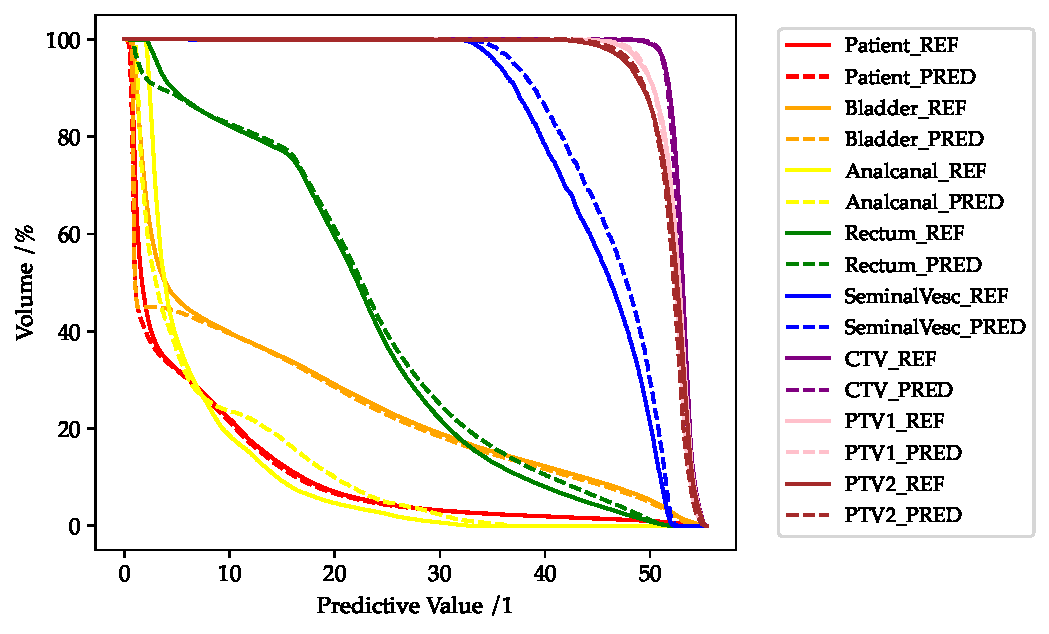
\includegraphics[width=\textwidth]{dvh.pdf}
    \caption{dvh for prostate cancer test plan with gamma passrate of 99.36.}\label{fig:dvh}
\end{figure}

\begin{figure}[ht]
    \centering
    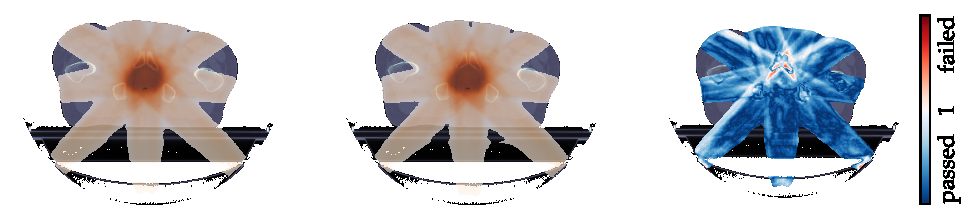
\includegraphics[width=\textwidth]{example_pt1.pdf}
    \caption{Dose prediction example on isocentric slice on prostate cancer patient from test cohort with prostate data only trained model. From left to right: target dose; dose prediction; gamma map for isocentric slice with a gamma pass rate of 98.02\%}
    \label{fig:prediction}
\end{figure}

\subsection{These 2 / Experiment 2}

The model shows rather poor translatability to other body regions. A summary over the prediction accuracy of the prostate only trained model for the tumor entities liver, mamma, H\&N and lmyphnodes is given in \autoref{tab:prost} gives a summary over. The model shows particular problems with breast cancer plans with a mean gamma passrate of 63.25~±~6.72\%. An examplary case is given by \autoref{fig:mamma_pred} showing low accuracy in the high dose aswell as lower dose areas of the volume. eingehen auf die werte kurz erklären

\begin{figure}[ht]
    \centering
    
\includegraphics[width=\textwidth]{example_mt1.pdf}
    \caption{Dose prediction example on isocentric slice on breast cancer patient from test cohort with prostate data only trained model. From left to right: target dose; dose prediction; gamma map for isocentric slice with a gamma pass rate of 53.78\%}
    \label{fig:mamma_pred}
\end{figure}

\begin{table}
    \centering
    \begin{tabular}{|ll|cccc|}
    \hline
                            &                      & \textbf{Liver} & \textbf{Mamma} & \textbf{H\&N} & \textbf{LK} \\ \hline
    Number of Patient Plans & /1                   & 5              & 5              & 5             & 15          \\ \cline{1-2}
    Mean Gamma Passrate     & \multirow{3}{*}{/\%} & 77.69          & 63.25          & 76.19         & 82.12       \\
    STD Gamma Passrate      &                      & 10.13          & 6.72           & 4.99          & 11.51       \\
    Median Gamma Passrate   &                      & 80.39          & 63.48          & 77.67         & 85.9        \\ \hline
    \end{tabular}
    \caption{Summary of gamma passrates for liver, mamma, head and lyphnodes tumor patients,  hier noch min max einfügen}
    \label{tab:prost}
\end{table}


\subsection{These 3 / Experiment 3}

The training of the network took around 9 days with a batchsize of 128 and $5.0\cdot10^5$ patches of size 32x32x32 voxels. The training was performced on 4 nvidia gtx 2080 ti and a initial learning rate of 10\textsuperscript{-4} decreasing by a factor  10 as soon as the validation loss or the gamma pass rate on the validation set did not decrease for 50 epochs. The training was stopped when no improvement was observed at a learning rate of 10\textsuperscript{-6} for 50 epochs. 

Model performance for prostate, liver, mamma and head tumor sites are summarized in . Auf die Werte eingehen kurz beschreiben

\begin{table}
    \centering
    \begin{tabular}{|ll|C{1.4cm}C{1.4cm}C{1.4cm}C{1.4cm}C{1.4cm}|}
    \hline
                            &                      & \multicolumn{1}{l}{\textbf{Prostate}} & \textbf{Liver} & \textbf{Mamma} & \textbf{H\&N} & \textbf{LN} \\ \hline
    Number of Patient Plans & /1                   & 5                                     & 5              & 5              & 5             & 15          \\ \cline{1-2}
    Mean Gamma Passrate     & \multirow{3}{*}{/\%} & 97.85                                 & 97.59          & 87.46          & 90.68         & 90.71       \\
    STD Gamma Passrate      &                      & 2.82                                  & 4.56           & 6.61           & 6.4           & 9.6         \\
    Median Gamma Passrate   &                      & 98.59                                 & 99.92          & 86.15          & 92.74         & 94.19       \\ \hline
    \end{tabular}
    \caption{Summary of gamma passrates for liver, mamma, head and lyphnodes tumor patients min max hinzufügen }
    \label{tab:mixed}
\end{table}

Comparing the two trained models shows a non significant accuracy decrease for prostate plans and very significant increases for the mixed aswell as the lymphnode test dataset (19.53\%, 8.59\% for mixed and lymphnode dataset respectively).

Comparing prostate only to mixed trained model is depictedd in fig. .... 

\begin{figure}[ht]
    \centering
    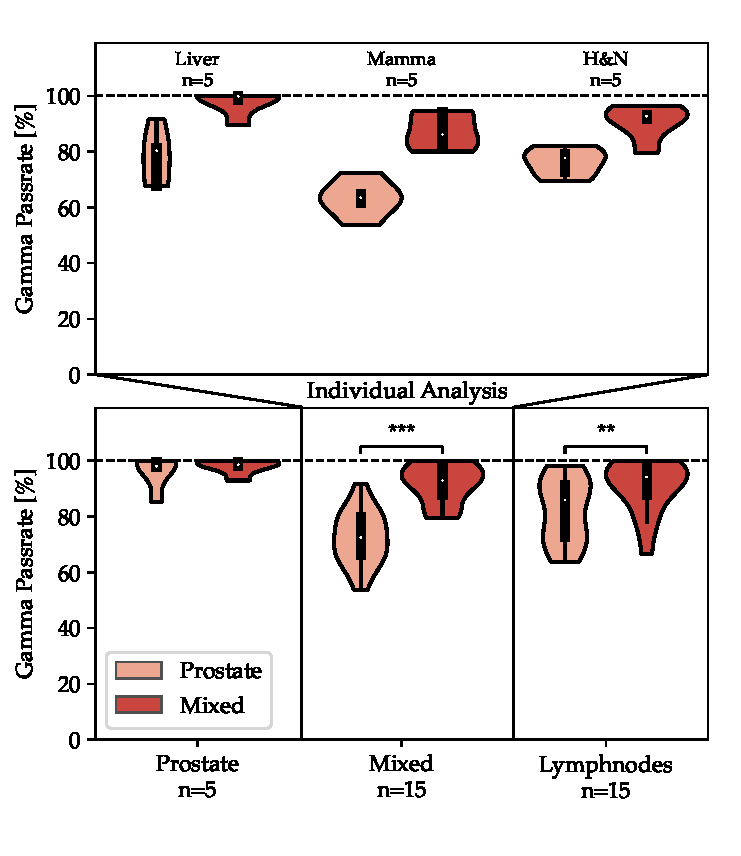
\includegraphics[width=0.7\textwidth]{plans.pdf}
    \caption{Prediction accuracy comparison between prostate only and mixed trained models. Passrates for liver, mamma and H\&N are combined into one group of `mixed' data. Significance level using a wilcoxon signed-ranked test are shown above the compared dataseries. zusätzlich plot für einzelne entities also leber, mamma, h\&N einzeln, sternchen erklären oder direkt obendrüber schreiben, feste convention finden wie ich die beiden Model nennen will}\label{fig:comparison}
\end{figure}

Single segment analysis gives a deeper insight into the actual performance differences of the model. we therefore assessed the gamma passrate for each single segment of all test data (fig ...). Additional information about performance regarding fieldsize can be benefitial to predict wether an unseen segment will reach high dose conformaty. fig ... shows the analysis for each segment of the test data regarding their fieldsize. additional information about the occurence of each discretized fieldsize range is shown in the background. 

\begin{figure}
    \centering
    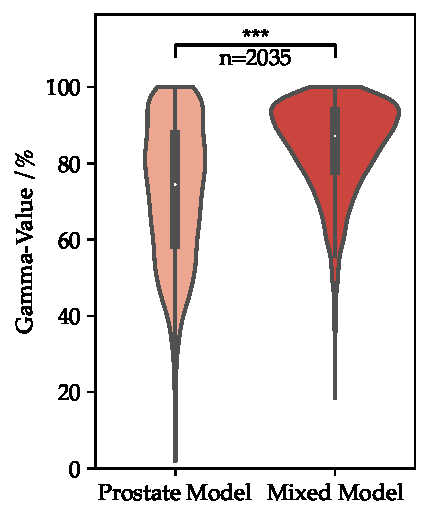
\includegraphics[width=0.5\textwidth]{segs_all.pdf}
    \caption{Prediction accuracy for all segments of the test data.}\label{fig:all_test}
\end{figure}

\begin{figure}
    \centering
    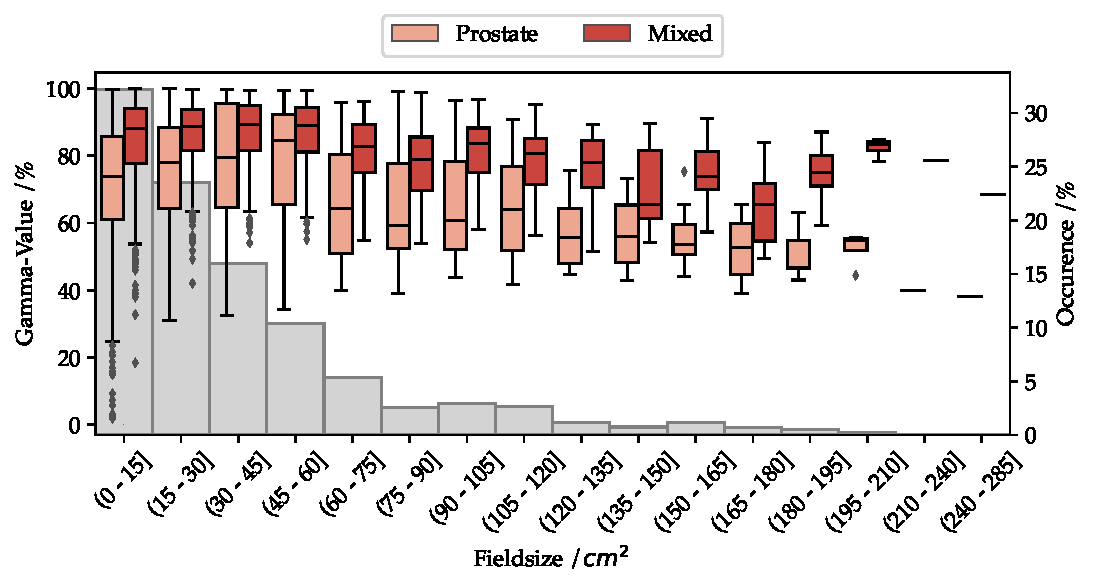
\includegraphics[width=\textwidth]{segs_fz_15.pdf}
    \caption{Prediction accuracy of each segment with respect to field size for prostate only and mixed trained model.}\label{fig:fz_test}
\end{figure}

\subsection{These 4 / Experiment 4}

Both models showed low gamma passrates for all waterslab positions tested. A summary of the accuracy is given in \autoref{tab:phantom_res}. The dose conformaty decreases with increasing phantom distance to the accelerator head for the prostate only trained model. The model which was trained on the mixed data set shows better passrates for all slab distances. The transversal view in \autoref{fig:phantom} shows that the prostate model is better at representing the peak at the beginning of the slab than the mixed model for a slab depth of 100 pixels. At higher slab distances the prostate model resembles the qualitative dose distribution quite well, while failing at reaching the correct predictive value. The mixed model can not reach the correct peak height at the beginning but predicts the later curve very well in terms of height and curvature in the transversal view. The coronal and sagital view both show that the penumbra is resembles very well by both models. At slab depths of 200 and 300 pixels the shoulders of the dose profile drop too fast for the mixed trained model in the coronal view. eingehen auf anstieg bei mixed model im randbereich

\begin{figure}
    \centering
    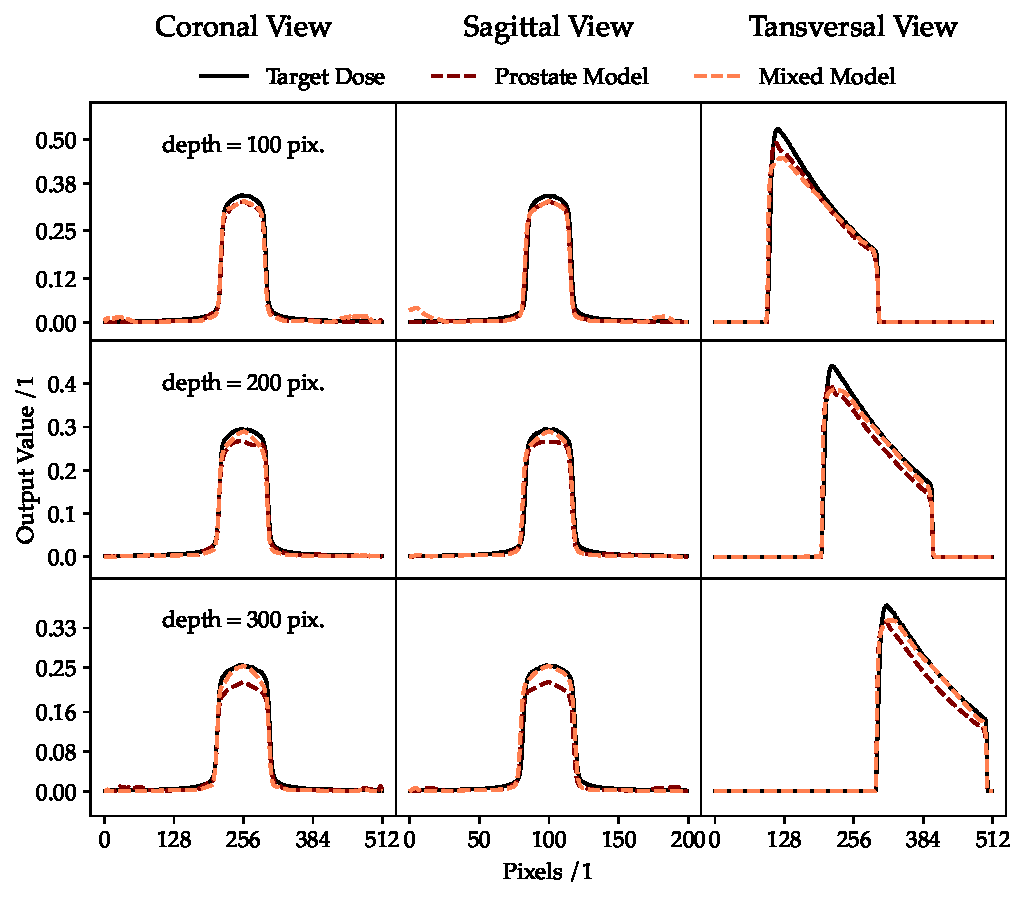
\includegraphics[width=\textwidth]{quer.pdf}
    \caption{Coronal, sagital and transversal view of the dose distributions for 100, 200 and 300 px depth in the phantom volume}\label{fig:phantom}
\end{figure}

\begin{table}[]
    \begin{tabular}{|lc|cc|cc|cc|}
    \hline
    Water slab position & /pixel & \multicolumn{2}{c|}{\textbf{100}} & \multicolumn{2}{c|}{\textbf{200}} & \multicolumn{2}{c|}{\textbf{300}} \\ \hline
    Model               &        & Mixed          & Prostate         & Mixed          & Prostate         & Mixed          & Prostate         \\
    Gamma Passrate      & /\%    & 60.122         & 56.080           & 45.539         & 27.713           & 48.427         & 19.246           \\ \hline
    \end{tabular}
    \caption{Gamma passrates for prostate only and mixed trained models for different water slab phantom positions inside an air volume. Water slab thickness was 200 pixels.}
    \label{tab:phantom_res}
\end{table}